\documentclass[a4paper,12pt]{article}
\usepackage{graphicx,amsfonts,url}
\usepackage[utf8]{inputenc}
\title{Using the Agent Simulator}
\author{}
\date{2013}

\setlength{\parindent}{0pt}
\setlength{\parskip}{2ex}

\begin{document}
\maketitle

\section*{Installation}

Please follow instructions specified for your platform.

\subsubsection*{GNU/Linux}

\begin{enumerate}
\item Using your distribution's package management system, install libraries SDL and SDL\_gfx.
In Ubuntu, libraries can be installed by issuing this command as user root:
\begin{verbatim}
# apt-get install libsdl1.2debian libsdl-gfx1.2-4
\end{verbatim}
In OpenSUSE, you can run this command:
\begin{verbatim}
# zypper install libSDL-1_2-0 libSDL_gfx13
\end{verbatim}
In Gentoo, this command will install the necessary packages:
\begin{verbatim}
# emerge -av media-libs/libsdl media-libs/sdl-gfx
\end{verbatim}

\item The directory in the second line of the file \texttt{run.lisp} must be changed to match the project root directory, e.g.
\begin{verbatim}
(cd "~/agentsim")
\end{verbatim}
\end{enumerate}

If you have 64-bit architecture and want to use 32-bit LispWorks Personal Edition, make sure you have the
libraries mentioned above compiled for the 32-bit architecture. You might have to compile the libraries for the
different architecture yourself.

\subsubsection*{Windows}
Libraries for the 32-bit architecture are bundled with this software. Just change the second line of the file
\texttt{run.lisp} to match the project root directory, e.g.
\begin{verbatim}
(cd "c:\\Users\\user\\Documents\\agentsim")
\end{verbatim}

\section*{Usage}
\begin{enumerate}
\item Load the file \texttt{run.lisp} in your favourite Common Lisp implementation. Tested working implementations
include LispWorks 6.1 Personal Edition on Windows and 32-bit GNU/Linux, CLISP on GNU/Linux and SBCL also on GNU/Linux. For
LispWorks 6.1 Personal Edition on 64-bit GNU/Linux see the note above.

\item Choose the game, you want to play, and run it. E.g. the game Hide\&seek with \texttt{ask-user-agent} can be started by:
\begin{verbatim}
(run-gui (make-hs-world6))
\end{verbatim}
Substitute \texttt{hs} with \texttt{tl} for Touch-last or \texttt{bs} for Blind-seek game.

\item Window shows up looking like Figure~\ref{fig:ask-user-agent}.

\begin{figure}\centering 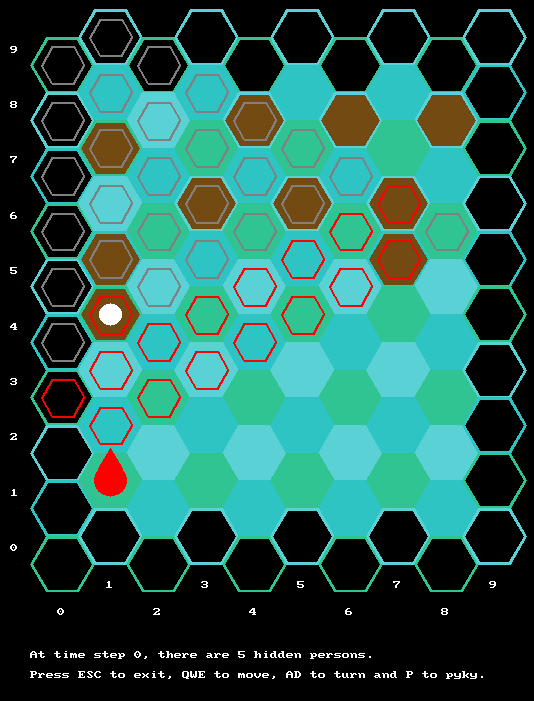
\includegraphics[width=0.8\textwidth]{images/ask-user-agent} \caption[Spuštění agenta
\texttt{ask-user-agent}.]{Running the \texttt{ask-user-agent}. Empty hexagons with red border mark a visible cell
	in percept. Grey border marks a cell in a shadow (\texttt{dark}).}\label{fig:ask-user-agent}
\end{figure}

\item In Hide\&seek, you can use keys $Q$, $W$ and $E$ to move north-west, north and north-east. Keys $A$ and $D$ turn
the agent to the left and to the right. Pressing $P$ causes the agent to pyky, $S$ stops the game. For details consult the rules of the
chosen game.
\end{enumerate}

\section*{Implementing your own agent}

\begin{enumerate}
\item Create a Lisp file for your agent in the directory \texttt{agent} with the name like
\texttt{hide-seek6-FITusername.lisp} and contents from the template as shown in the game file, e.g.
\texttt{hex/hide-seek6.lisp}.

\item Inside the game file, e.g. \texttt{hex/hide-seek6.lisp}, change the environment definition at the top to 
include your agent instead of the \texttt{ask-user-agent}.

\item Add a line to load the file containing your agent to the file \texttt{loadfiles.lisp}. Then load \texttt{run.lisp}
	or just \texttt{loadfiles.lisp}, if you have already loaded \texttt{run.lisp} before.
\item Start the simulation with your agent by running e.g.:
\begin{verbatim}
(run-gui (make-hs-world6))
\end{verbatim}

\item You can now see, what your agent does at each time step. Control the simulation by performing one of the following actions:
\begin{enumerate}
\item Press \emph{Escape} to exit the simulation.
\item Press numeric keys \emph{1} to \emph{9} to forward the time by $n$ steps.
\item Press \emph{0} to forward the time by $10$ steps.
\item Press \emph{H} to forward the time by $100$ (\emph{H}undred) steps.
\item Press \emph{T} to forward the time by $1000$ (\emph{T}housand) steps.
\item Pressing any other key will forward the time by $1$ step.
\end{enumerate}


\end{enumerate}

\end{document}

